%% flowchart.tex --- ratvalue: Model Flowchart
%% Compile: lualatex flowchart.tex

\documentclass[11pt, a4paper, landscape]{article}
\usepackage[utf8]{inputenc}
\usepackage[T1]{fontenc}
\usepackage[english]{babel}
\usepackage[margin=1.1cm]{geometry}
\usepackage{tikz}
\usetikzlibrary{arrows.meta, calc}
\usepackage{lmodern}
\usepackage{amsmath}
\usepackage{xcolor}

%% Palette
\colorlet{Ci}{blue!12}       \colorlet{Bi}{blue!55!black}
\colorlet{Cc}{green!13}      \colorlet{Bc}{green!45!black}
\colorlet{Co}{yellow!25}     \colorlet{Bo}{orange!75!black}
\colorlet{Ca}{violet!10}     \colorlet{Ba}{violet!70!black}
\colorlet{Cgr}{gray!7}       \colorlet{Bgr}{gray!45}

\tikzset{
  inp/.style  = {draw=Bi, fill=Ci, thick, rounded corners=3pt,
                 minimum width=3.5cm, minimum height=0.62cm,
                 align=center, font=\small, inner sep=3pt},
  cmp/.style  = {draw=Bc, fill=Cc, thick, rounded corners=3pt,
                 minimum width=3.5cm, minimum height=0.62cm,
                 align=center, font=\small, inner sep=3pt},
  res/.style  = {draw=Bo, fill=Co, thick, rounded corners=3pt,
                 minimum width=3.5cm, minimum height=0.62cm,
                 align=center, font=\small, inner sep=3pt},
  altm/.style  = {draw=Ba, fill=Ca, thick, rounded corners=3pt,
                 minimum width=3.0cm, minimum height=0.72cm,
                 align=center, font=\small, inner sep=3pt},
  grp/.style  = {draw=Bgr, fill=Cgr, dashed, thick, rounded corners=5pt},
  arr/.style  = {-{Stealth[length=5pt]}, thick, Bgr},
  arrd/.style = {-{Stealth[length=5pt]}, thick, Ba!75, dashed},
}

\pagestyle{empty}
\begin{document}
\begin{center}

{\large\bfseries ratvalue\enspace---\enspace Computational Graph}\\[0.2em]
{\small\itshape
Damodaran valuation framework $\cdot$ C++23 $\cdot$
solid arrows = exact rational arithmetic,\enspace
dashed arrows = shared infrastructure (double discounting)}\\[0.7em]

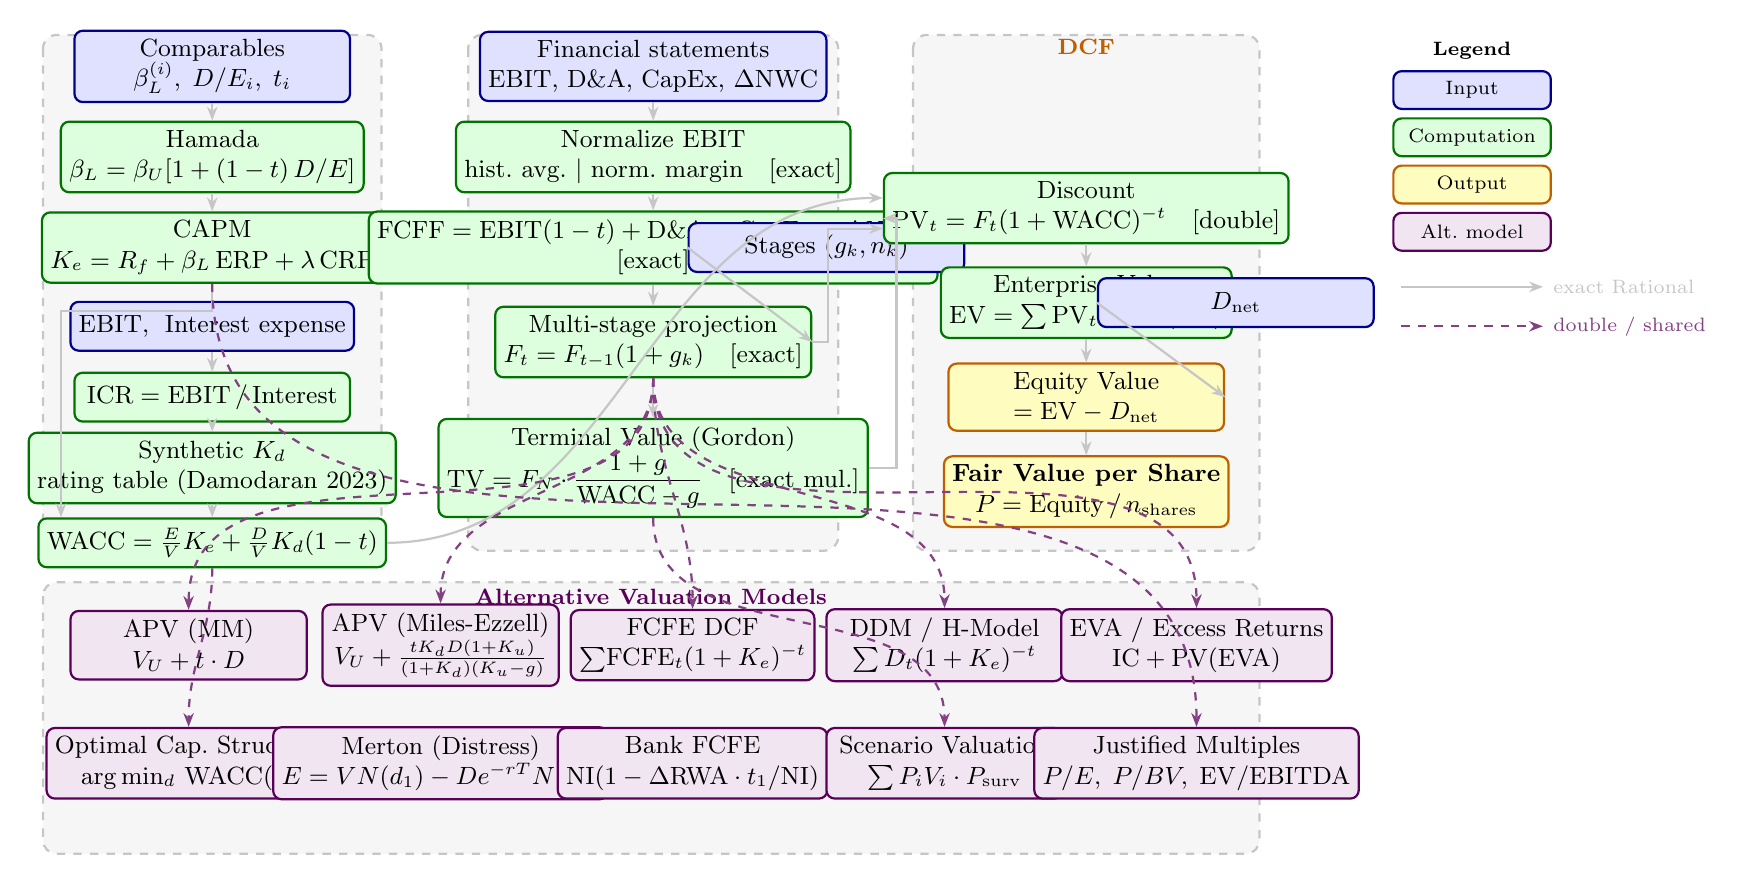
\begin{tikzpicture}[x=1cm, y=1.0cm]

%%──────────────────────────────────────────────────
%% Group backgrounds
%%──────────────────────────────────────────────────
\draw[grp] (-0.35,0.4) rectangle (3.95,-6.15);
\node[font=\footnotesize\bfseries, text=Bi] at (1.8,0.25) {Cost of Capital};

\draw[grp] (5.05,0.4) rectangle (9.75,-6.15);
\node[font=\footnotesize\bfseries, text=Bc] at (7.4,0.25) {Cash Flows};

\draw[grp] (10.7,0.4) rectangle (15.1,-6.15);
\node[font=\footnotesize\bfseries, text=Bo] at (12.9,0.25) {DCF};

\draw[grp] (-0.35,-6.55) rectangle (15.1,-10.0);
\node[font=\footnotesize\bfseries, text=Ba] at (7.37,-6.73)
  {Alternative Valuation Models};

%%──────────────────────────────────────────────────
%% COLUMN A: Cost of Capital
%%──────────────────────────────────────────────────
\node[inp] (rawbeta) at (1.8,0.0)
  {Comparables\\$\beta_L^{(i)},\;D/E_i,\;t_i$};

\node[cmp] (hamada) at (1.8,-1.15)
  {Hamada\\$\beta_L = \beta_U[1+(1-t)\,D/E]$};

\node[cmp] (capm) at (1.8,-2.3)
  {CAPM\\$K_e = R_f + \beta_L\,\mathrm{ERP} + \lambda\,\mathrm{CRP}$};

\node[inp] (finkd) at (1.8,-3.3)
  {EBIT,\; Interest expense};

\node[cmp] (icr) at (1.8,-4.2)
  {$\mathrm{ICR} = \mathrm{EBIT}\,/\,\mathrm{Interest}$};

\node[cmp] (kd) at (1.8,-5.1)
  {Synthetic $K_d$\\rating table (Damodaran 2023)};

\node[cmp] (wacc) at (1.8,-6.05)
  {$\mathrm{WACC} = \tfrac{E}{V}K_e + \tfrac{D}{V}K_d(1-t)$};

\draw[arr] (rawbeta) -- (hamada);
\draw[arr] (hamada)  -- (capm);
\draw[arr] (finkd)   -- (icr);
\draw[arr] (icr)     -- (kd);
\draw[arr] (kd)      -- (wacc);
\draw[arr] (capm.south) -- ++(0,-0.35) -| ($(wacc.north west)+(0.3,0)$);

%%──────────────────────────────────────────────────
%% COLUMN B: Cash Flows
%%──────────────────────────────────────────────────
\node[inp] (stmts) at (7.4,0.0)
  {Financial statements\\EBIT, D\&A, CapEx, $\Delta$NWC};

\node[cmp] (norm) at (7.4,-1.15)
  {Normalize EBIT\\hist.\ avg.\ $|$\ norm.\ margin\quad[exact]};

\node[cmp] (fcff) at (7.4,-2.3)
  {$\mathrm{FCFF} = \mathrm{EBIT}(1-t)+\mathrm{D\&A}-\mathrm{CapEx}-\Delta\mathrm{NWC}$\\{[exact]}};

\node[inp] (gstage) at (9.6,-2.3)
  {Stages $(g_k,n_k)$};

\node[cmp] (proj) at (7.4,-3.5)
  {Multi-stage projection\\$F_t = F_{t-1}(1+g_k)$\quad[exact]};

\node[cmp] (tv) at (7.4,-5.1)
  {Terminal Value (Gordon)\\$\mathrm{TV}=F_N\cdot\dfrac{1+g}{\mathrm{WACC}-g}$\quad[exact mul.]};

\draw[arr] (stmts)      -- (norm);
\draw[arr] (norm)       -- (fcff);
\draw[arr] (fcff)       -- (proj);
\draw[arr] (gstage.west) -- (proj.east);
\draw[arr] (proj)       -- (tv);

%%──────────────────────────────────────────────────
%% COLUMN C: DCF
%%──────────────────────────────────────────────────
\node[cmp] (pv) at (12.9,-1.8)
  {Discount\\$\mathrm{PV}_t = F_t(1+\mathrm{WACC})^{-t}$\quad[double]};

\node[cmp] (ev) at (12.9,-3.0)
  {Enterprise Value\\$\mathrm{EV} = \sum\mathrm{PV}_t + \mathrm{PV(TV)}$};

\node[inp] (dnet) at (14.8,-3.0)
  {$D_{\mathrm{net}}$};

\node[res] (eqv) at (12.9,-4.2)
  {Equity Value\\$= \mathrm{EV} - D_{\mathrm{net}}$};

\node[res] (price) at (12.9,-5.4)
  {\bfseries Fair Value per Share\\$P = \mathrm{Equity}\,/\,n_{\mathrm{shares}}$};

\draw[arr] (pv)      -- (ev);
\draw[arr] (dnet.west) -- (eqv.east);
\draw[arr] (ev)      -- (eqv);
\draw[arr] (eqv)     -- (price);

%% Cross-column: cash flows + WACC → discount
\draw[arr] (tv.east)      -- ++(0.35,0) |- ($(pv.west)+(0,-0.13)$);
\draw[arr] (proj.east)    -- ++(0.2,0)  |- ($(pv.west)+(0,-0.26)$);
\draw[arr] (wacc.east)    to[out=0,in=180] ($(pv.west)+(0,0.13)$);

%%──────────────────────────────────────────────────
%% ALTERNATIVE MODELS — two rows
%%──────────────────────────────────────────────────
%% Row 1  y = -7.35
\node[altm] (apvmm)   at (1.5 , -7.35)
  {APV (MM)\\$V_U + t\cdot D$};
\node[altm] (apvme)   at (4.7 , -7.35)
  {APV (Miles-Ezzell)\\$V_U + \tfrac{tK_d D(1+K_u)}{(1+K_d)(K_u-g)}$};
\node[altm] (fcfedcf) at (7.9 , -7.35)
  {FCFE DCF\\$\sum\!\mathrm{FCFE}_t(1+K_e)^{-t}$};
\node[altm] (ddmh)    at (11.1, -7.35)
  {DDM / H-Model\\$\sum D_t(1+K_e)^{-t}$};
\node[altm] (eva)     at (14.3, -7.35)
  {EVA / Excess Returns\\$\mathrm{IC}+\mathrm{PV(EVA)}$};

%% Row 2  y = -8.85
\node[altm] (capst)   at (1.5 , -8.85)
  {Optimal Cap.\ Structure\\$\arg\min_d\,\mathrm{WACC}(d)$};
\node[altm] (mert)    at (4.7 , -8.85)
  {Merton (Distress)\\$E=VN(d_1)-De^{-rT}N(d_2)$};
\node[altm] (bank)    at (7.9 , -8.85)
  {Bank FCFE\\$\mathrm{NI}(1-\Delta\mathrm{RWA}\cdot t_1/\mathrm{NI})$};
\node[altm] (scen)    at (11.1, -8.85)
  {Scenario Valuation\\$\sum P_i V_i\cdot P_{\mathrm{surv}}$};
\node[altm] (relat)   at (14.3, -8.85)
  {Justified Multiples\\$P/E,\;P/BV,\;\mathrm{EV/EBITDA}$};

%% Dashed arrows (shared infrastructure)
\draw[arrd] (proj.south) to[out=-90,in=90] (apvmm.north);
\draw[arrd] (proj.south) to[out=-90,in=90] (apvme.north);
\draw[arrd] (proj.south) to[out=-90,in=90] (fcfedcf.north);
\draw[arrd] (proj.south) to[out=-90,in=90] (ddmh.north);
\draw[arrd] (proj.south) to[out=-90,in=90] (eva.north);
\draw[arrd] (tv.south)   to[out=-90,in=90] (scen.north);
\draw[arrd] (wacc.south) to[out=-90,in=90] (capst.north);
\draw[arrd] (capm.south) to[out=-90,in=90] (relat.north);

%%──────────────────────────────────────────────────
%% Legend
%%──────────────────────────────────────────────────
\node[inp, minimum width=2.0cm, minimum height=0.48cm,
     font=\scriptsize] at (17.8,-0.3) {Input};
\node[cmp, minimum width=2.0cm, minimum height=0.48cm,
     font=\scriptsize] at (17.8,-0.9) {Computation};
\node[res, minimum width=2.0cm, minimum height=0.48cm,
     font=\scriptsize] at (17.8,-1.5) {Output};
\node[altm, minimum width=2.0cm, minimum height=0.48cm,
     font=\scriptsize] at (17.8,-2.1) {Alt.\ model};
\node[font=\scriptsize\bfseries]   at (17.8, 0.2) {Legend};

\draw[arr]  (16.9,-2.8) -- ++(1.8,0)
  node[right,font=\scriptsize]{exact Rational};
\draw[arrd] (16.9,-3.3) -- ++(1.8,0)
  node[right,font=\scriptsize]{double / shared};

\end{tikzpicture}

\vspace{0.25em}
{\scriptsize
\textbf{Exact:} \texttt{Rational} or \texttt{Currency::scale} --- no floating-point rounding.
\quad
\textbf{Double:} discount factors $(1+r)^{-t}$ via \texttt{std::pow}; PV sums accumulated in \texttt{double}.
\quad
TV multiplier $\tfrac{1+g}{r-g}$ is computed as exact \texttt{Rational}
\emph{before} the double discounting step.
}

\end{center}
\end{document}
